
\section{Laser stand for the MAPMT characterization}
The large number of the channels in the RICH detector  poses challenging problem for the MAPMT testing and calibration.
RICH consists of 391 MAPMTs resulting in total number of channels equal to 25024. So in order to test them efficiently within a reasonable timeframe the fully automated test stand was build to evaluate 6 MAPMTs at once, as shown on Fig.~\ref{fig:MAPMTtest}.

\begin{figure}[hbt]
	\centering
	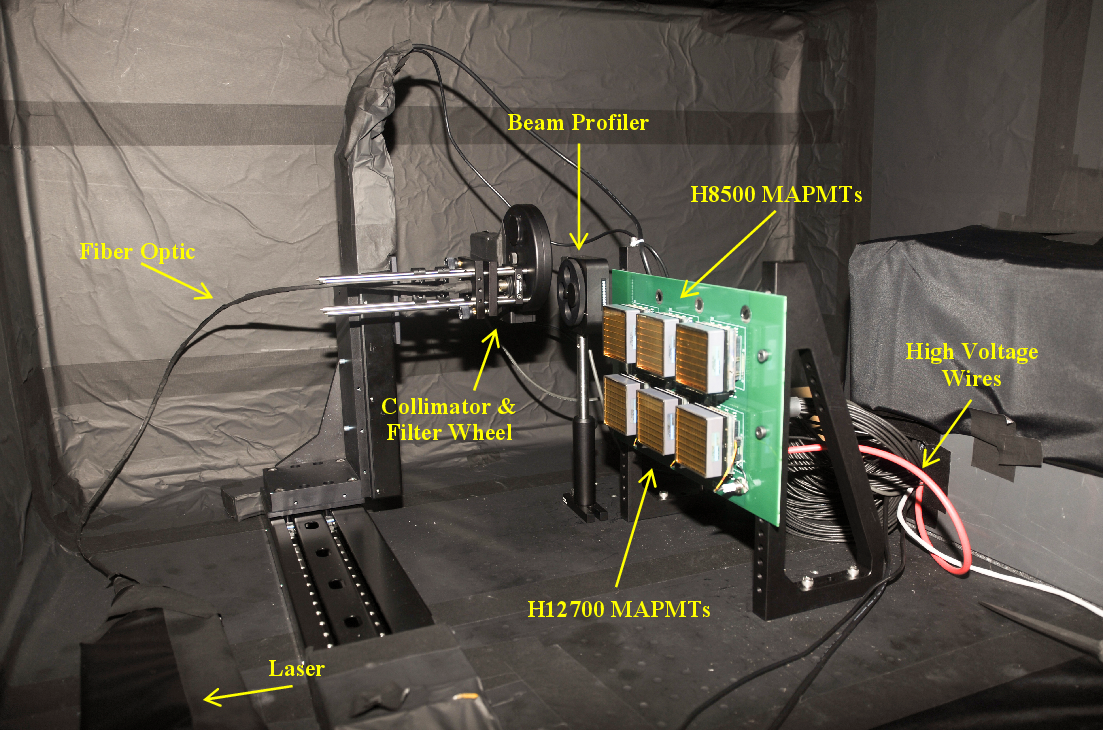
\includegraphics[width=0.9\linewidth]{figures/blackbox.png}
	\caption{Inner view of the laser stand.}
	\label{fig:MAPMTtest}
\end{figure}

The test stand consists of picosecond diode  laser PiL047X with 470 nm wavelength, 2 long travel motorized stands to drive laser fiber in two dimensional space for individual pixel illumination, the motorized wheel with neutral density filter system, 2 adapter boards for MAPMT with JLab designed front-end electronics boards \cite{}{Contalbrigo:2020}.
The laser light is directed through the fiber and attenuated to the single photon level using the neutral density filters to mimic the conditions of the RICH detector.
The motors were remotely controlled to move the focused laser beam across (see Fig.~\ref{fig:beamopt1}) the entire surface of the MAPMT entrance window and illuminate one by one of all its 64 pixels individually.
Another option is to illuminate the whole surface of MAPMT photocathode at once using the Engineered Diffuser to produce square pattern with non-Gaussian intensity distribution (see Fig.~\ref{fig:beamopt2}). 

All laser stand equipment is sitting in the black box with non-reflective black material on the optical table. The laser interlock safety box automatically switch off laser, as well as front-end low voltage  electronics and MAPMT high voltage to prevent the possible photomultiplier damage or laser light human illumination in case if somebody will try to open the front door of the black box during the measurements.

\begin{figure}[bt]
	\centering
	\begin{subfigure}[b]{0.628\linewidth}
		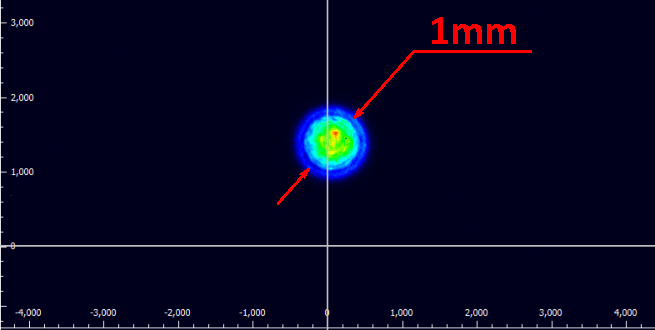
\includegraphics[width=\linewidth]{figures/beamspot.pdf}
		\caption{Focused laser beam with the dimension much less than the  MAPMT pixel size.}
		\label{fig:beamopt1}
	\end{subfigure}
	\begin{subfigure}[b]{0.354\linewidth}
		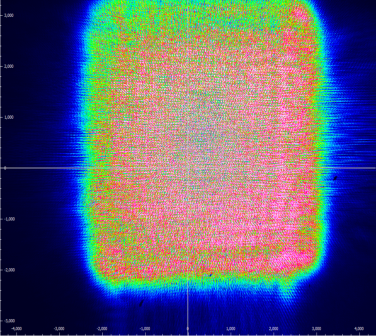
\includegraphics[width=\linewidth]{figures/beamsquare.pdf}
		\caption{Square pattern illuminated all MAPMT surface.}
		\label{fig:beamopt2}
	\end{subfigure}
	\caption{The laser light output options.}
\end{figure}

This configuration brings routine workload to minimum allowing the evaluation of 6 MAPMTs (equivalent to 328 conventional PMTs!) at 4 different high voltages and 6 different light intensities within 6 hours with less than 15 minutes of human intervention needed to load the MAPMTs to the front-end boards.

\begin{figure}[b]
	\centering
	\begin{subfigure}{0.3\linewidth}
		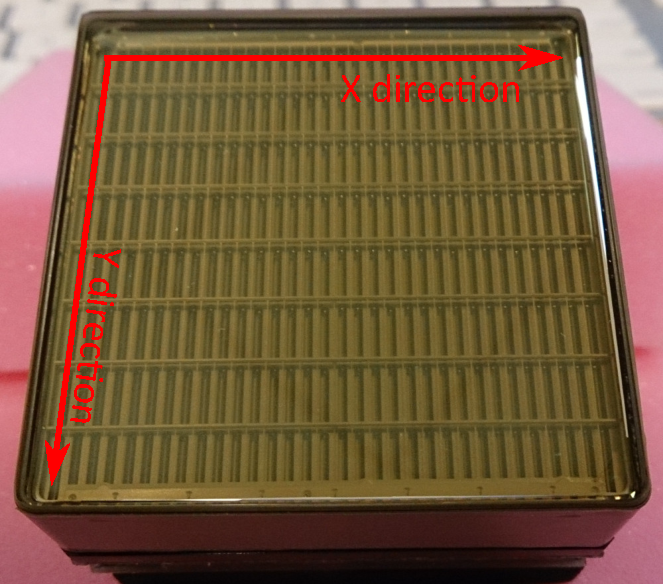
\includegraphics[width=\linewidth]{figures/surfaceuniform1.pdf}
		\caption{MAPMT with visible internal structure of metal channel dynodes and focusing mesh.}
		\label{fig:surfaceuniform1}
	\end{subfigure}
	\quad
	\begin{subfigure}{0.3\linewidth}
		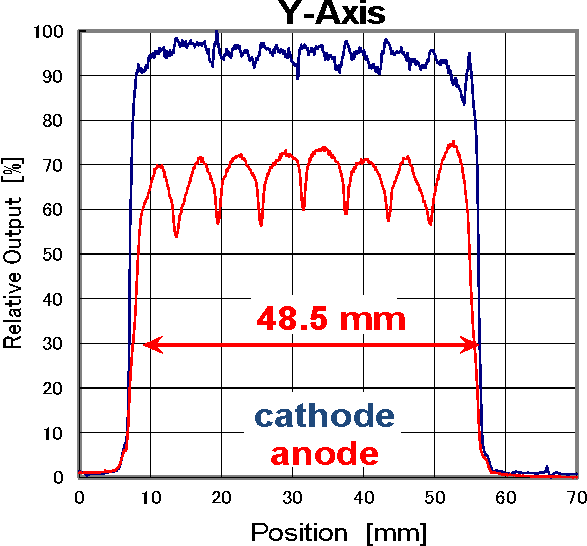
\includegraphics[width=\linewidth]{figures/surfaceuniform3.pdf}
		\caption{The response along the X axis; the signal drops in the deadspace between the pixels.}
		\label{fig:surfaceuniform2}
	\end{subfigure}
	\quad
	\begin{subfigure}{0.3\linewidth}
		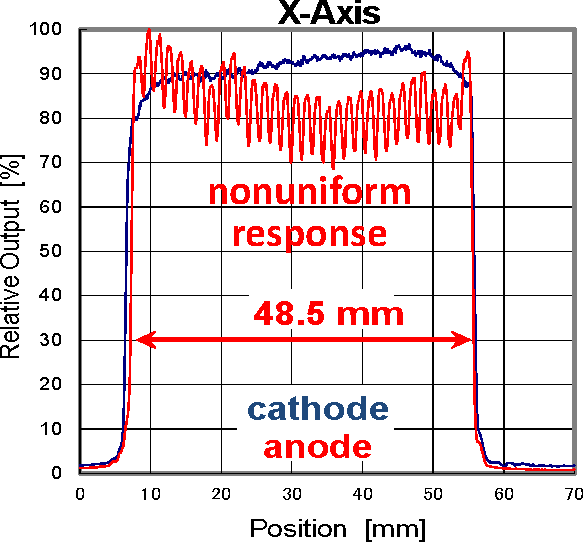
\includegraphics[width=\linewidth]{figures/surfaceuniform2.pdf}
		\caption{The response along the Y axis: multiple segmentations within the pixels.}
		\label{fig:surfaceuniform3}
	\end{subfigure}
	\caption{The response uniformity of MAPMT.}
	\label{fig:surfaceuniform}
\end{figure}


Before starting the systematic study of the MAPMT responses, a finer two dimensional scan of several pixels was performed in order to verify the uniformity of the response across pixel's surfaces, as shown on Fig.~\ref{fig:surfaceuniform}.
The horizontal and vertical axes denote laser beam position during the scan.
Along the both directions there are obvious drops in efficiency when the laser strikes the space between the pixels.
The drops are relatively narrow so the dead-space is very small as expected from the Hamamatsu specifications.
Additionally, a vertical efficiency variation is visible across the pixel in horizontal scan.
These inhomogeneities are correlated with the vertical walls separating dynode chains, owing to the constructional features of the MAPMT. The discontinuity in dynode structure is visible  on Fig.~\ref{fig:surfaceuniform1}.
The separate response maps for photocathode shows relatively uniform signal without efficiency drops, confirming that the variation arises from the dynode system.

\section*{Front-end electronics}

The highly integrated front-end electronics with modular design was developed for a large array of MAPMT H12700 to minimize the impact of the electronics material on the detector downstream the RICH.
An architecture of the readout electronics consists of front-end cards with dedicated Application Specific Integrated Circuit (ASIC) configured, controlled and readout by programmable devices such as Field Programmable Gate Array (FPGA).
The ASIC board is based on the MAROC3 integrated circuit whose excellent single photon capabilities both in analog and binary mode have been confirmed.
The final design has consists of stacked PCB layers behind each MAPMT sensor (see~Fig.~\ref{fig:feboards}).
The first layer houses the ASIC front end and ancillary components (e.g. external amplifier) and it is directly connected to the anodes array.
A second PCB will host the FPGA in charge of configuring, managing and acquiring one or more ASICs and the low voltage and HV bias distribution.
The use of the JLab SSP as controller and collector of the front-end data provides a strong synergy with the current JLab upgrade activity.
Data are transmitted on high speed serial (optical) lines minimizing the wiring and therefore the material budget.
With that sandwich architecture the total photon detection surface will be covered by a fixed number of basic units or tiles made up by two or three sensor each.
The total spacing for electronics will not exceed 20 cm in depth (including MAPMT and mechanical support).
The three-tiles electronics module with and without 3 H12700 MAPMTs installed is shown on~Fig.~\ref{fig:feboards}.

\begin{figure}[htb]
  \centering
  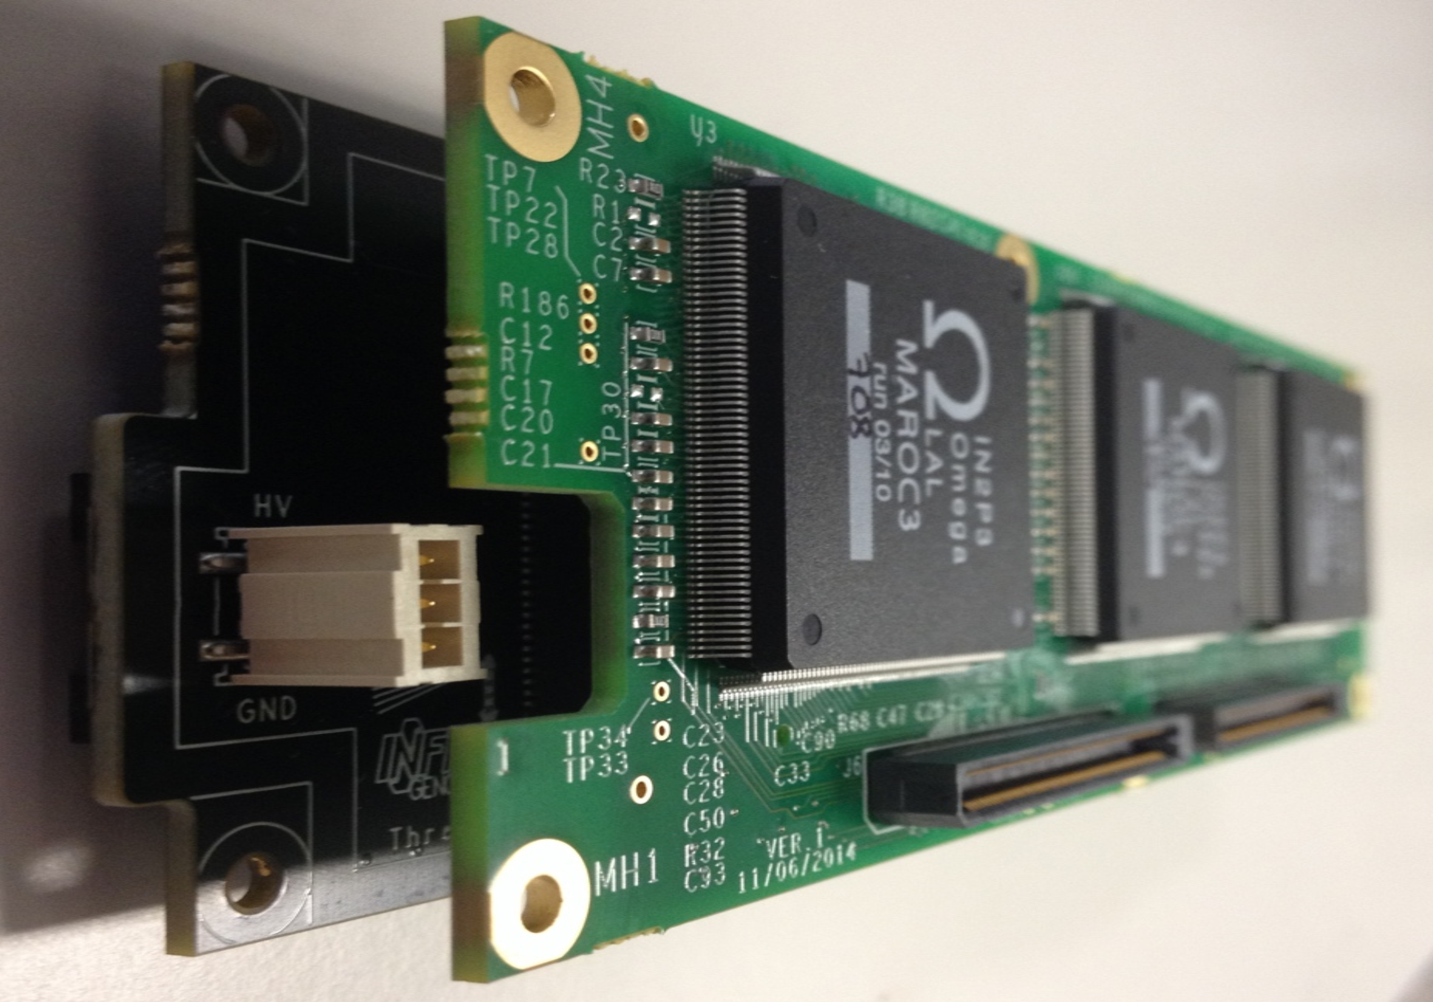
\includegraphics[width=0.9\linewidth]{figures/fe1.pdf}
  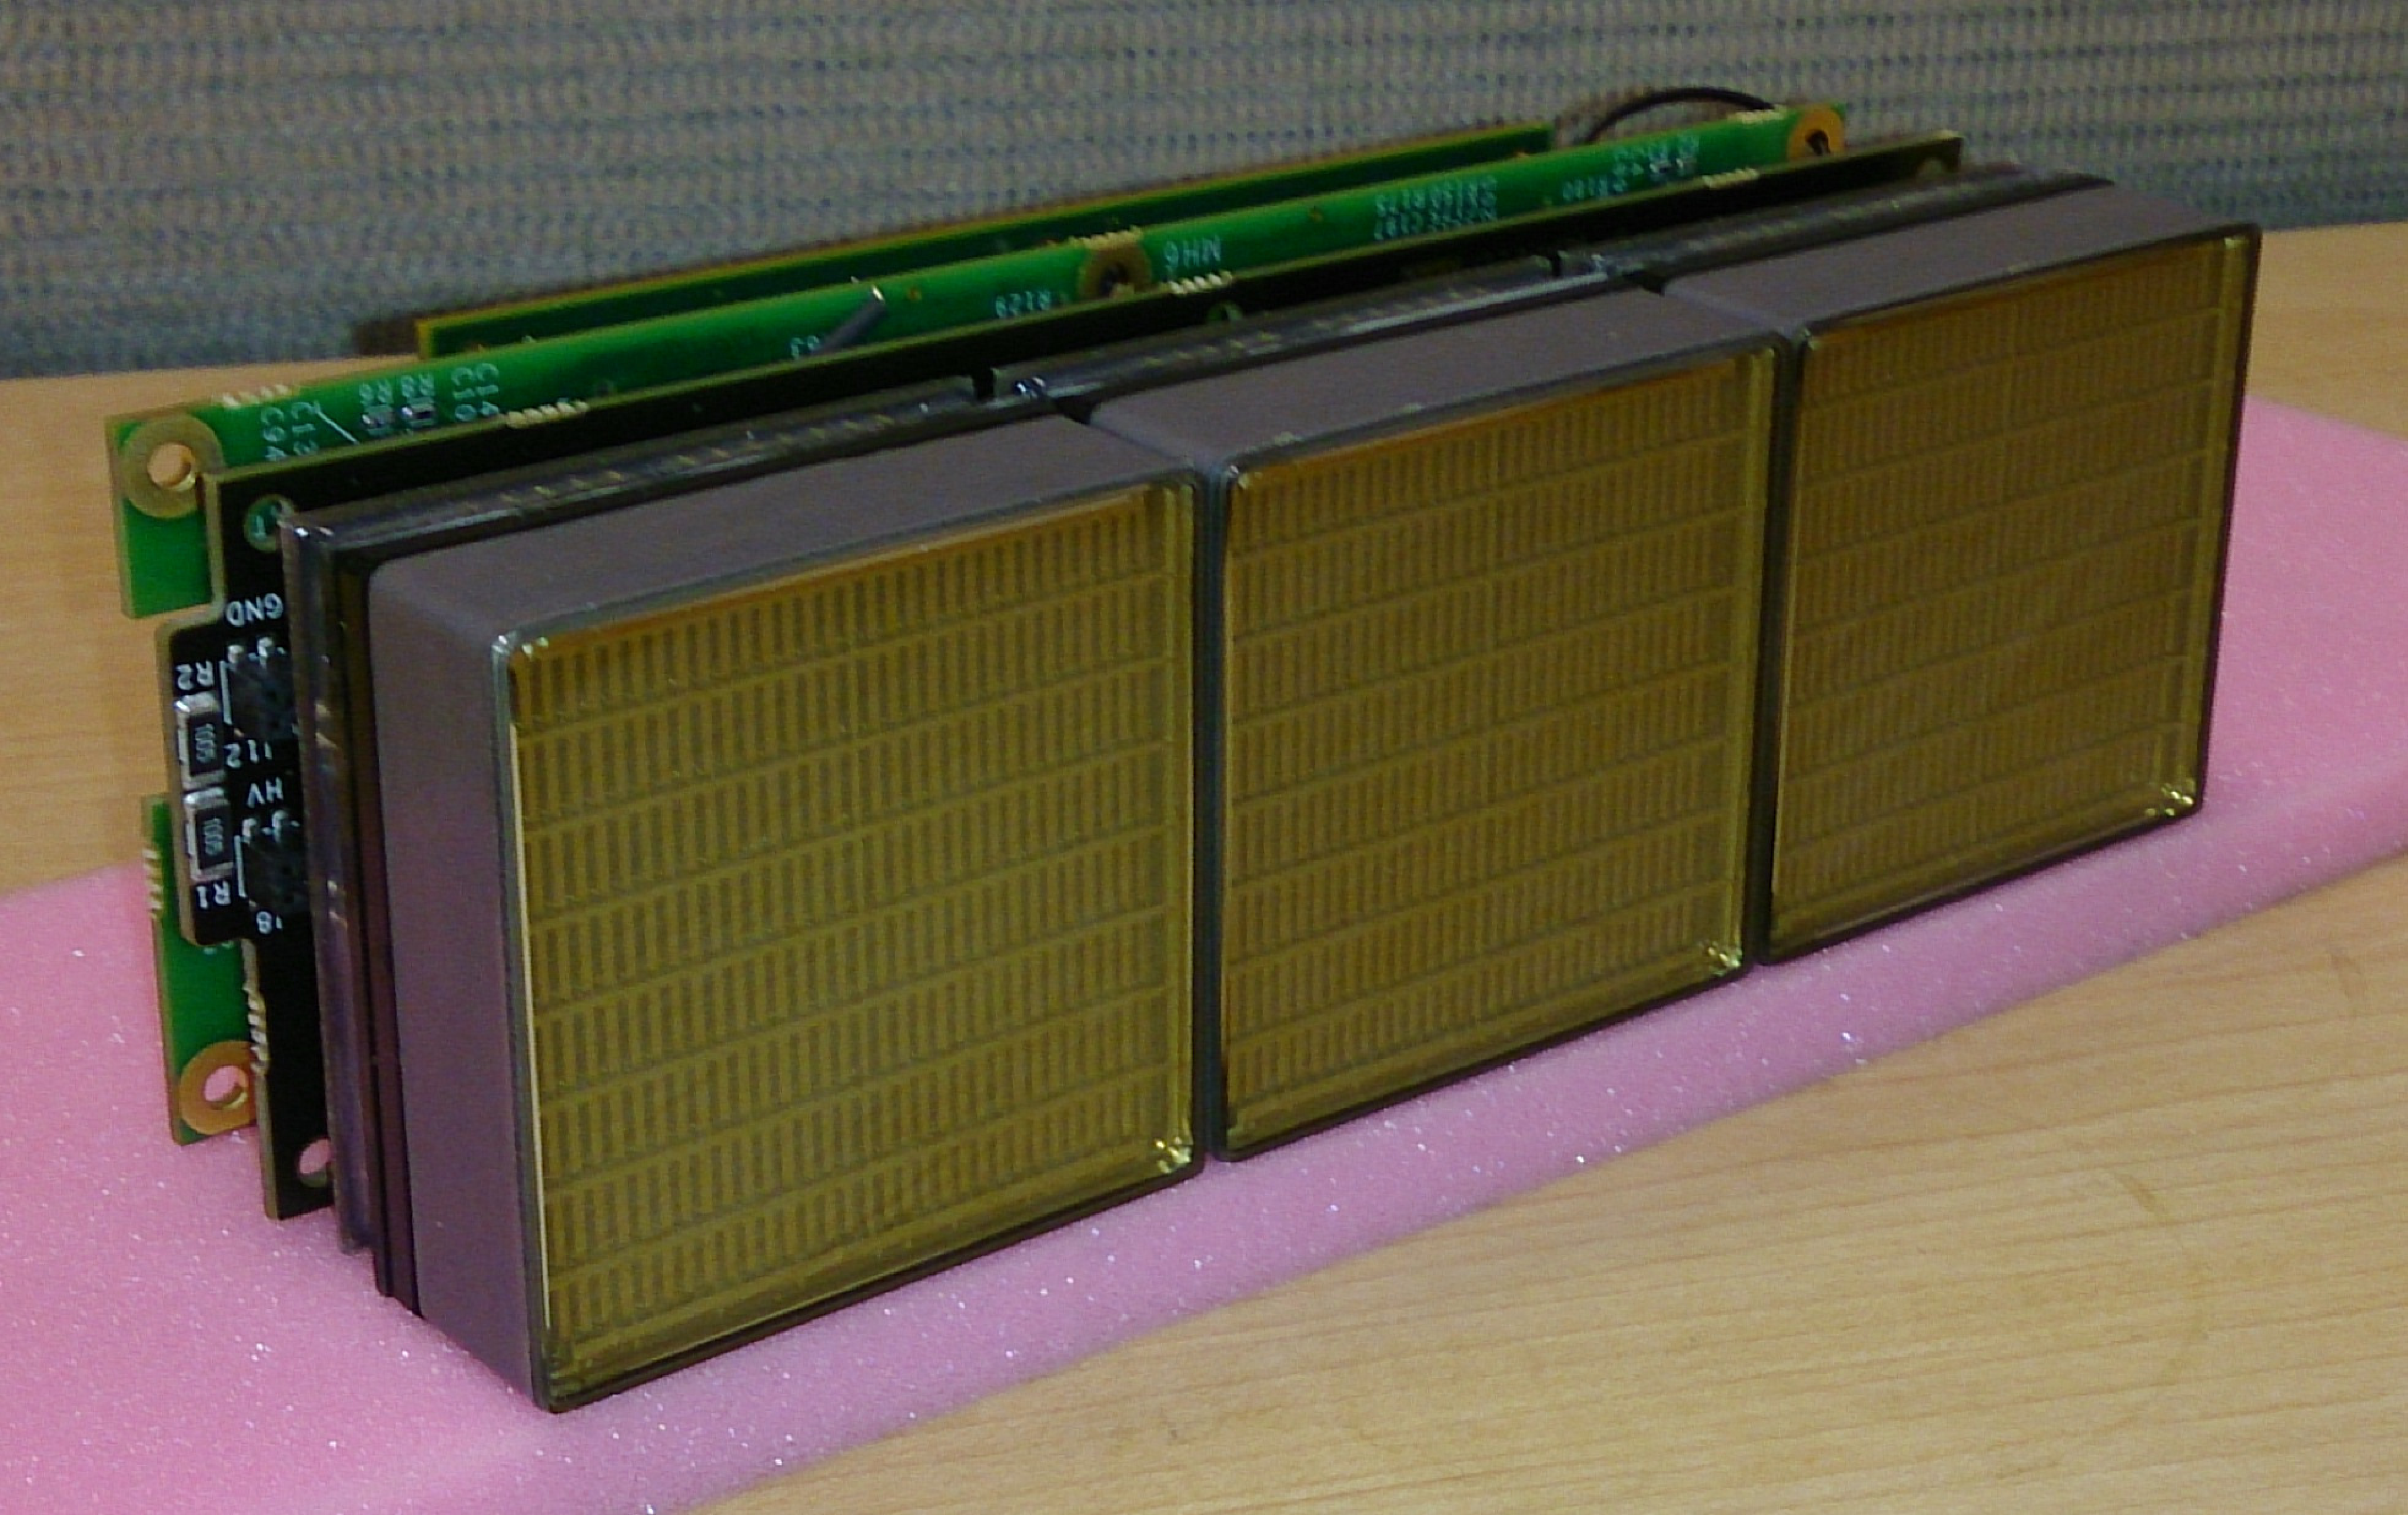
\includegraphics[width=0.9\linewidth]{figures/frontendPMT.pdf}
  \caption{Front-end electronics readout board and mounted MAPMTs.}
  \label{fig:feboards}
\end{figure}

The MAROC chip consists of 64 independent channels.
The single channel has a pre-amplification and configurable 8 bit gain correction stage followed by independent binary and analog lines.
The binary line is digital and most suitable for the RICH application.
We are planning to analyze the performance of MAROC chip as a function of its threshold and gain.
Additionally front-end electronics stability and noise will be tested as well.


\section*{Front-End Electronics for RICH}


Due to the high number of active channels in readout subsystem of the RICH detector and available limited space the Multi Anode ReadOut Chips (MAROC) were chosen to construct highly integrated front-end electronics with modular design.
The MAROC performances were checked and found suitable for the RICH requirements.
Each chip is equipped with single channel adjustable preamplifier, configurable signal shaping, slow shaper capable of charge measurements and binary output with fast shaping and adjustable threshold.
The custom modular design as shown on Fig.~\ref{fig:FEpics} consists of sandwich architecture where one board hosts the ASIC chips (2 or 3 per board) and another active board hosts the FPGA to manage and configure the ASICs, the third board is a passive adapter for MAPMT sockets.
It satisfies the following requirements:
\begin{itemize}
\item 100\% efficiency at 1/3 of single photoelectron signal (50 fC)
\item time resolution of 1 ns
\item short deadtime to sustain the trigger rate of 20 kHz
\item latency of 8 $\mu s$
\end{itemize}
The conceptual design of the electronics readout boards was finished in the RICH development phase and currently we have several board implementations available at Jefferson Lab and INFN for final tests.

The preliminary measurements with internal onboard charge injector, external charge injector and signal generator were performed to test and calibrate FE electronics.
However, the measurements of custom front-end electronics together with installed MAPMTs in the RICH Black Box setup are crucial for understanding the their future performance in the RICH detector in CLAS12.
RICH MAPMT test setup was modified to house two FE board at once inside the black box as shown on Fig.~\ref{fig:FEmount}.
The focus of the modification was to adapt the test setup in such way that the swap of FE boards would be fast and easy.
The PCB guidelines were installed inside the black box to ensure easy mounting and dismounting procedure universal for both 2-MAPMT and 3-MAPMT FE modules.
This requirement exists in light of the future measurements that our group is expected to perform on all FE modules for testing purposes.
Each FE module is connected to the low voltage power supply to power FPGA and ASIC boards. The communication between FPGA board and PC is performed using TCP/IP protocol via optical fiber network cable.
The HV cables, one per each module, supply power for attached MAPMTs.
The Data Acquision program runs on external PC under Linux OS, configures FPGA and MAROC boards and collects the data through the network interface.
As before the laser with neutral density filters and light diffuser is installed on moving platform to allow illumination of individual MAPMTs with different light intensities.
The current setup allows fast evaluation of FE modules with highly automatized procedure which is important because RICH will be utilizing 113 tiles with 3 MAPMTs and 23 tiles with 2 MAPMTs FE modules to house 391 MAPMTs.

The planned measurements will group individual boards with MAPMTs and treat them as a inseparable unit that will go into the final assembly of RICH detector.
Every unit will be tested in the black box setup to mimic the conditions of SPE regime expected during the RICH routine operations.
The calibration procedures will be developed and evaluated during these test measurements.
The gain equalization, individual channel amplification parameters and optimal threshold values will be investigated and resolved.
In addition, self-triggering capabilities of FE modules allow careful dark current measurements.
The previous measurements and evaluation of MAPMTs with different readout systems (JLab FADC) will be compared with FE measurements to better understand the MAPMTs and FE performances.
The calibration procedures will be developed and evaluated during these test measurements.

\begin{figure}[hbt]
  \centering
  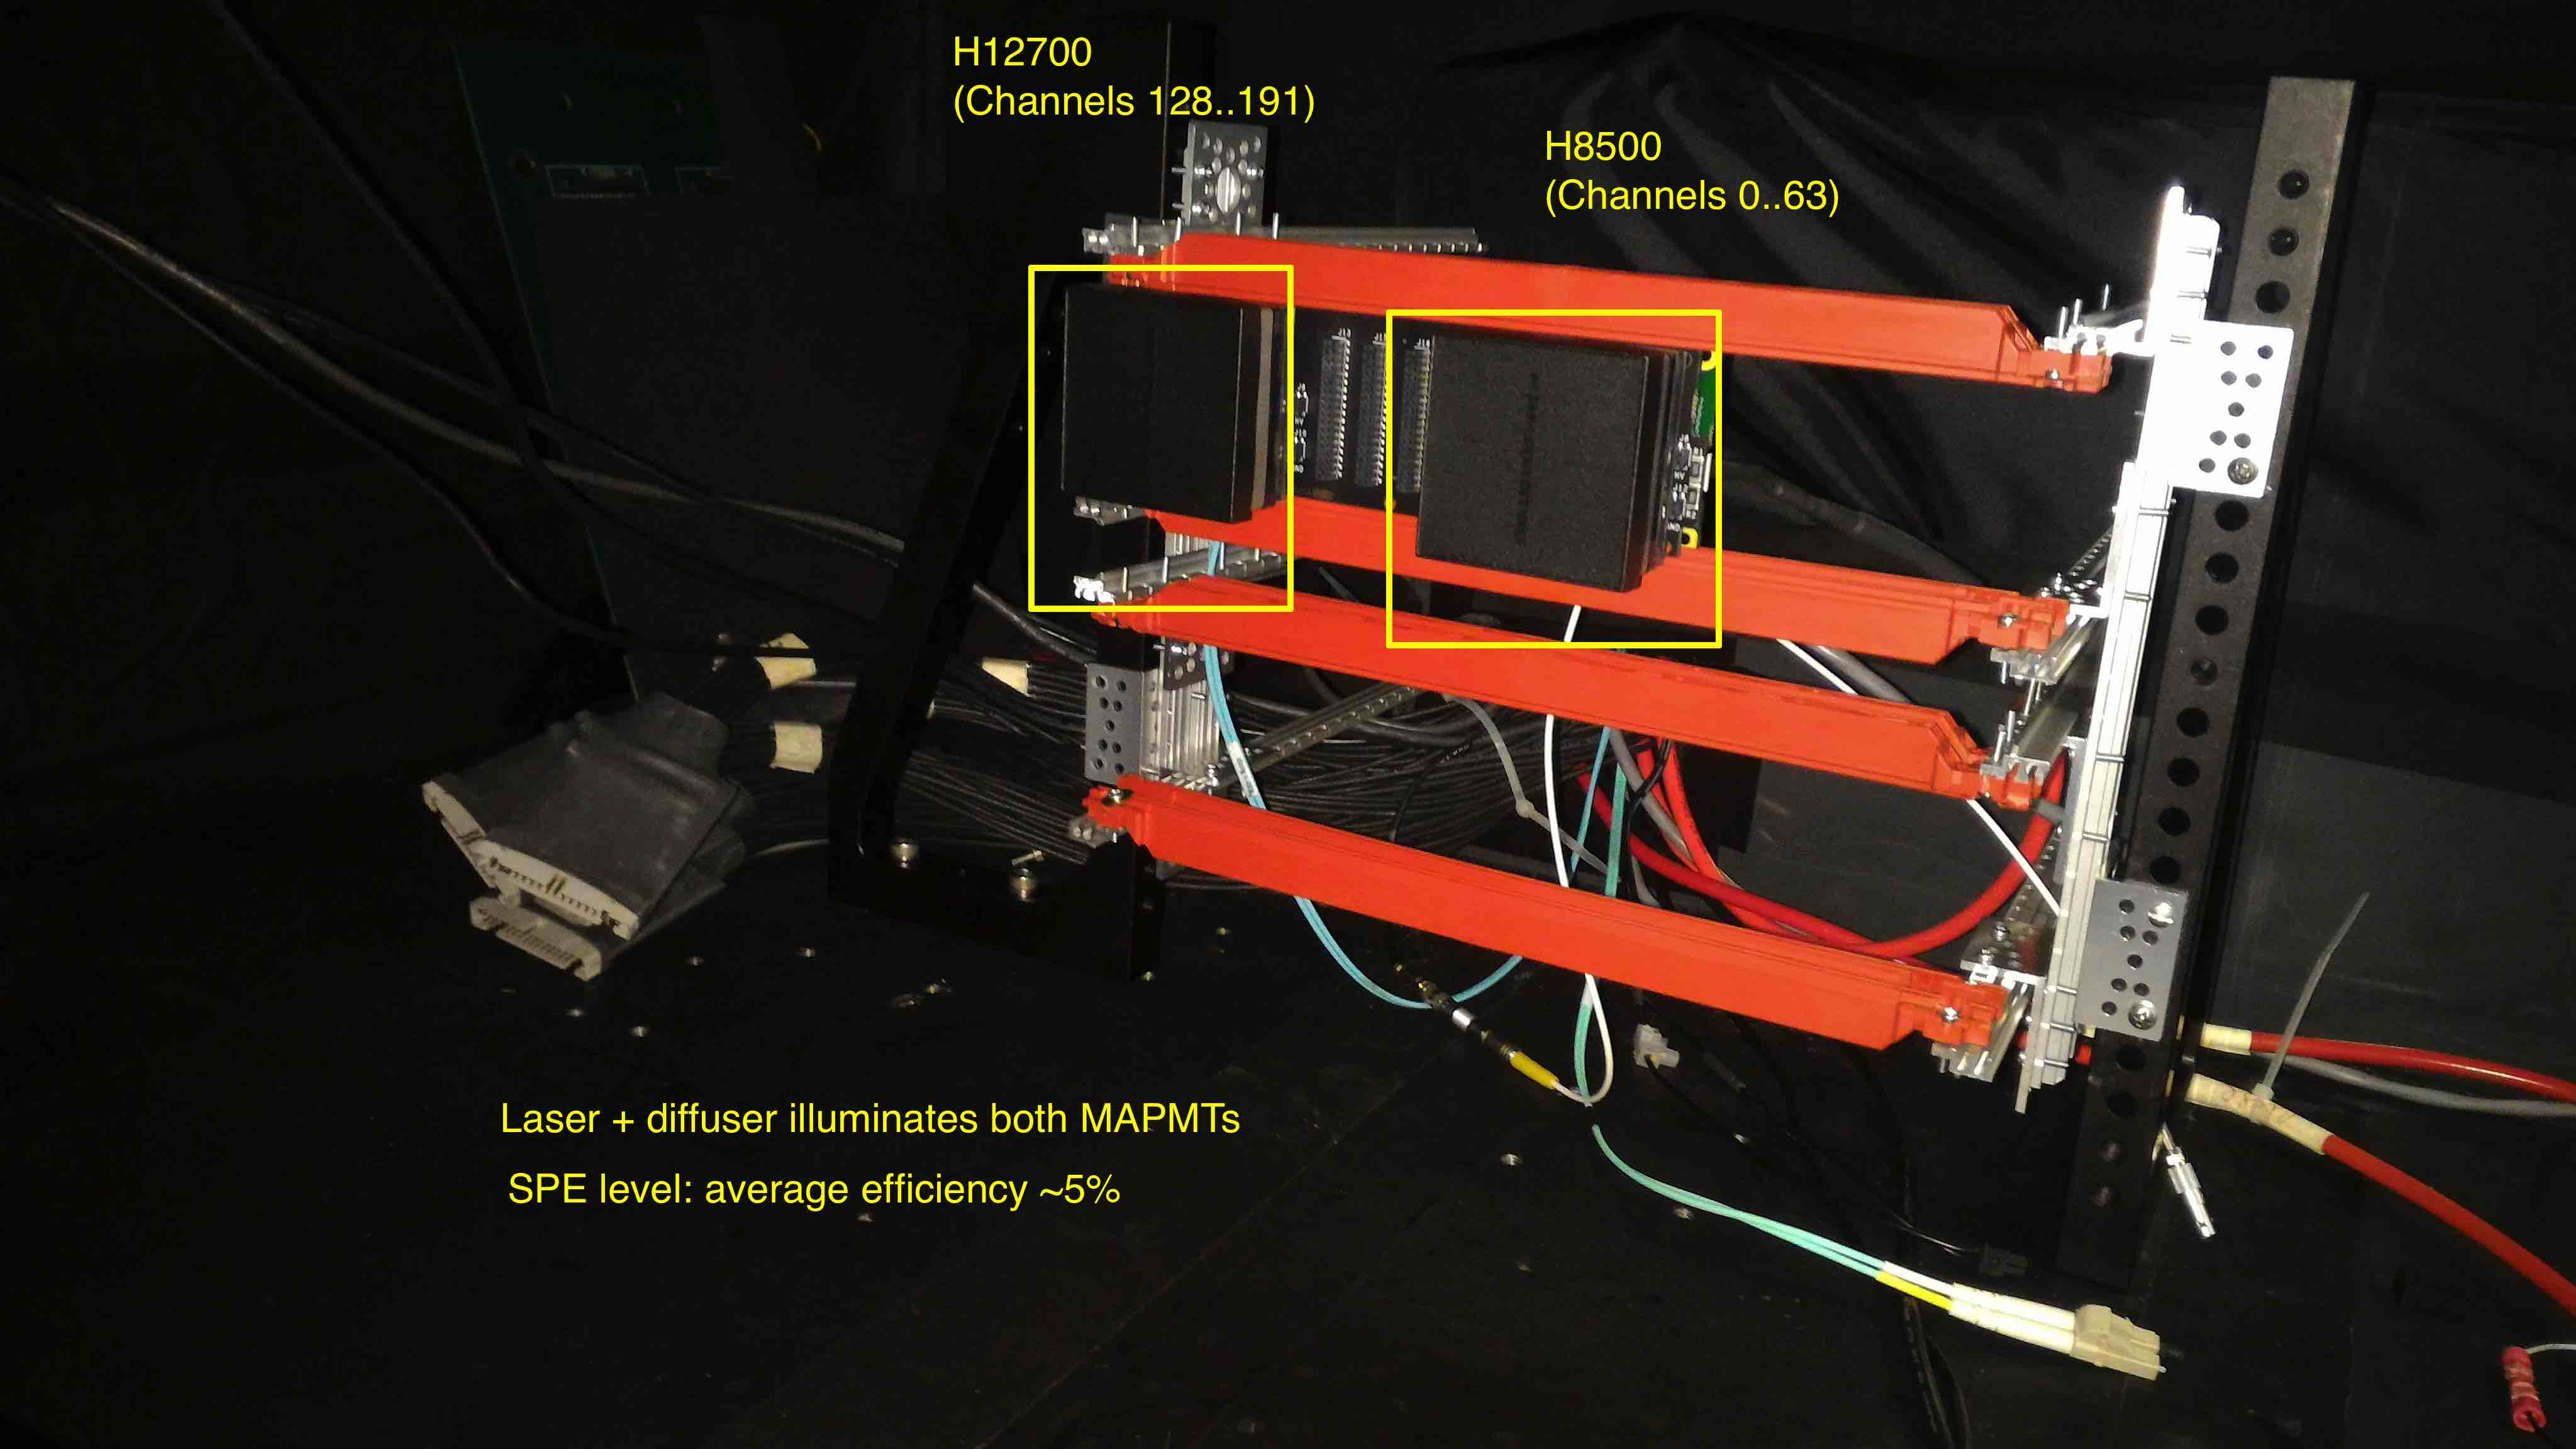
\includegraphics[width=0.9\linewidth]{figures/LaserSetup.jpg}
  \caption{Mount inside RICH Black box is capable to hold two Front-End boards and up to 6 MAPMTs}
  \label{fig:FEmount}
\end{figure}

The MAROC chip used to read MAPMT outputs has two main paths to feed the preamplified input current:
\begin{itemize}
\item analog line with a slow shaper which allow the injected charge measurements
\item binary line with a fast shaper followed by a discriminator with configurable threshold which allows to deliver trigger outputs
\end{itemize}
Both lines are independent and highly configurable.
The slow shaper can not be used during normal operation of RICH detector due to relatively small HOLD latency of 200 ns.
It can, however, be used for calibration purposes.
On the other hand the digital line with fast shaper is suitable for RICH operation and will be used to detect signals from Cherenkov photons incident on the readout panel.

The preliminary measurements of MAPMTs signal were taken using the FE tile with 3-MAPMTs installed inside the RICH black box.
Both lines were evaluated as shown of Fig.~\ref{fig:slowWaveform} and~\ref{fig:fastWaveform}
The internal pulse generator was used to trigger laser through its adjustable external trigger input achieving synchronization between light source and MAROC readout.
Then the data were collected with both lines collecting data in parallel.
Fig.~\ref{fig:slowMAROC} shows the slow shaper waveform for different charge injections from MAROC3 datasheet.
On the right Fig.~\ref{fig:slowJLab} shows the same waveform obtained from the data collected at Jefferson Lab using RICH test setup with laser and MAPMT.
In order to reconstruct the waveform of the slow shaper, the hold delays parameters was changed from 1 to 100 and data were collected at different values.
This measurements alow us to find the best value of the hold delay for internal ADC conversions which correpond to the signal maximum at around (13 ticks = 104 ns).
It ensures the largest precision to the charge measurements.
The shape of the analog output waveform is configurable and its gain and peaking speed can be changed.


\begin{figure}[hbt]
	\centering
	\begin{subfigure}{0.49\linewidth}
		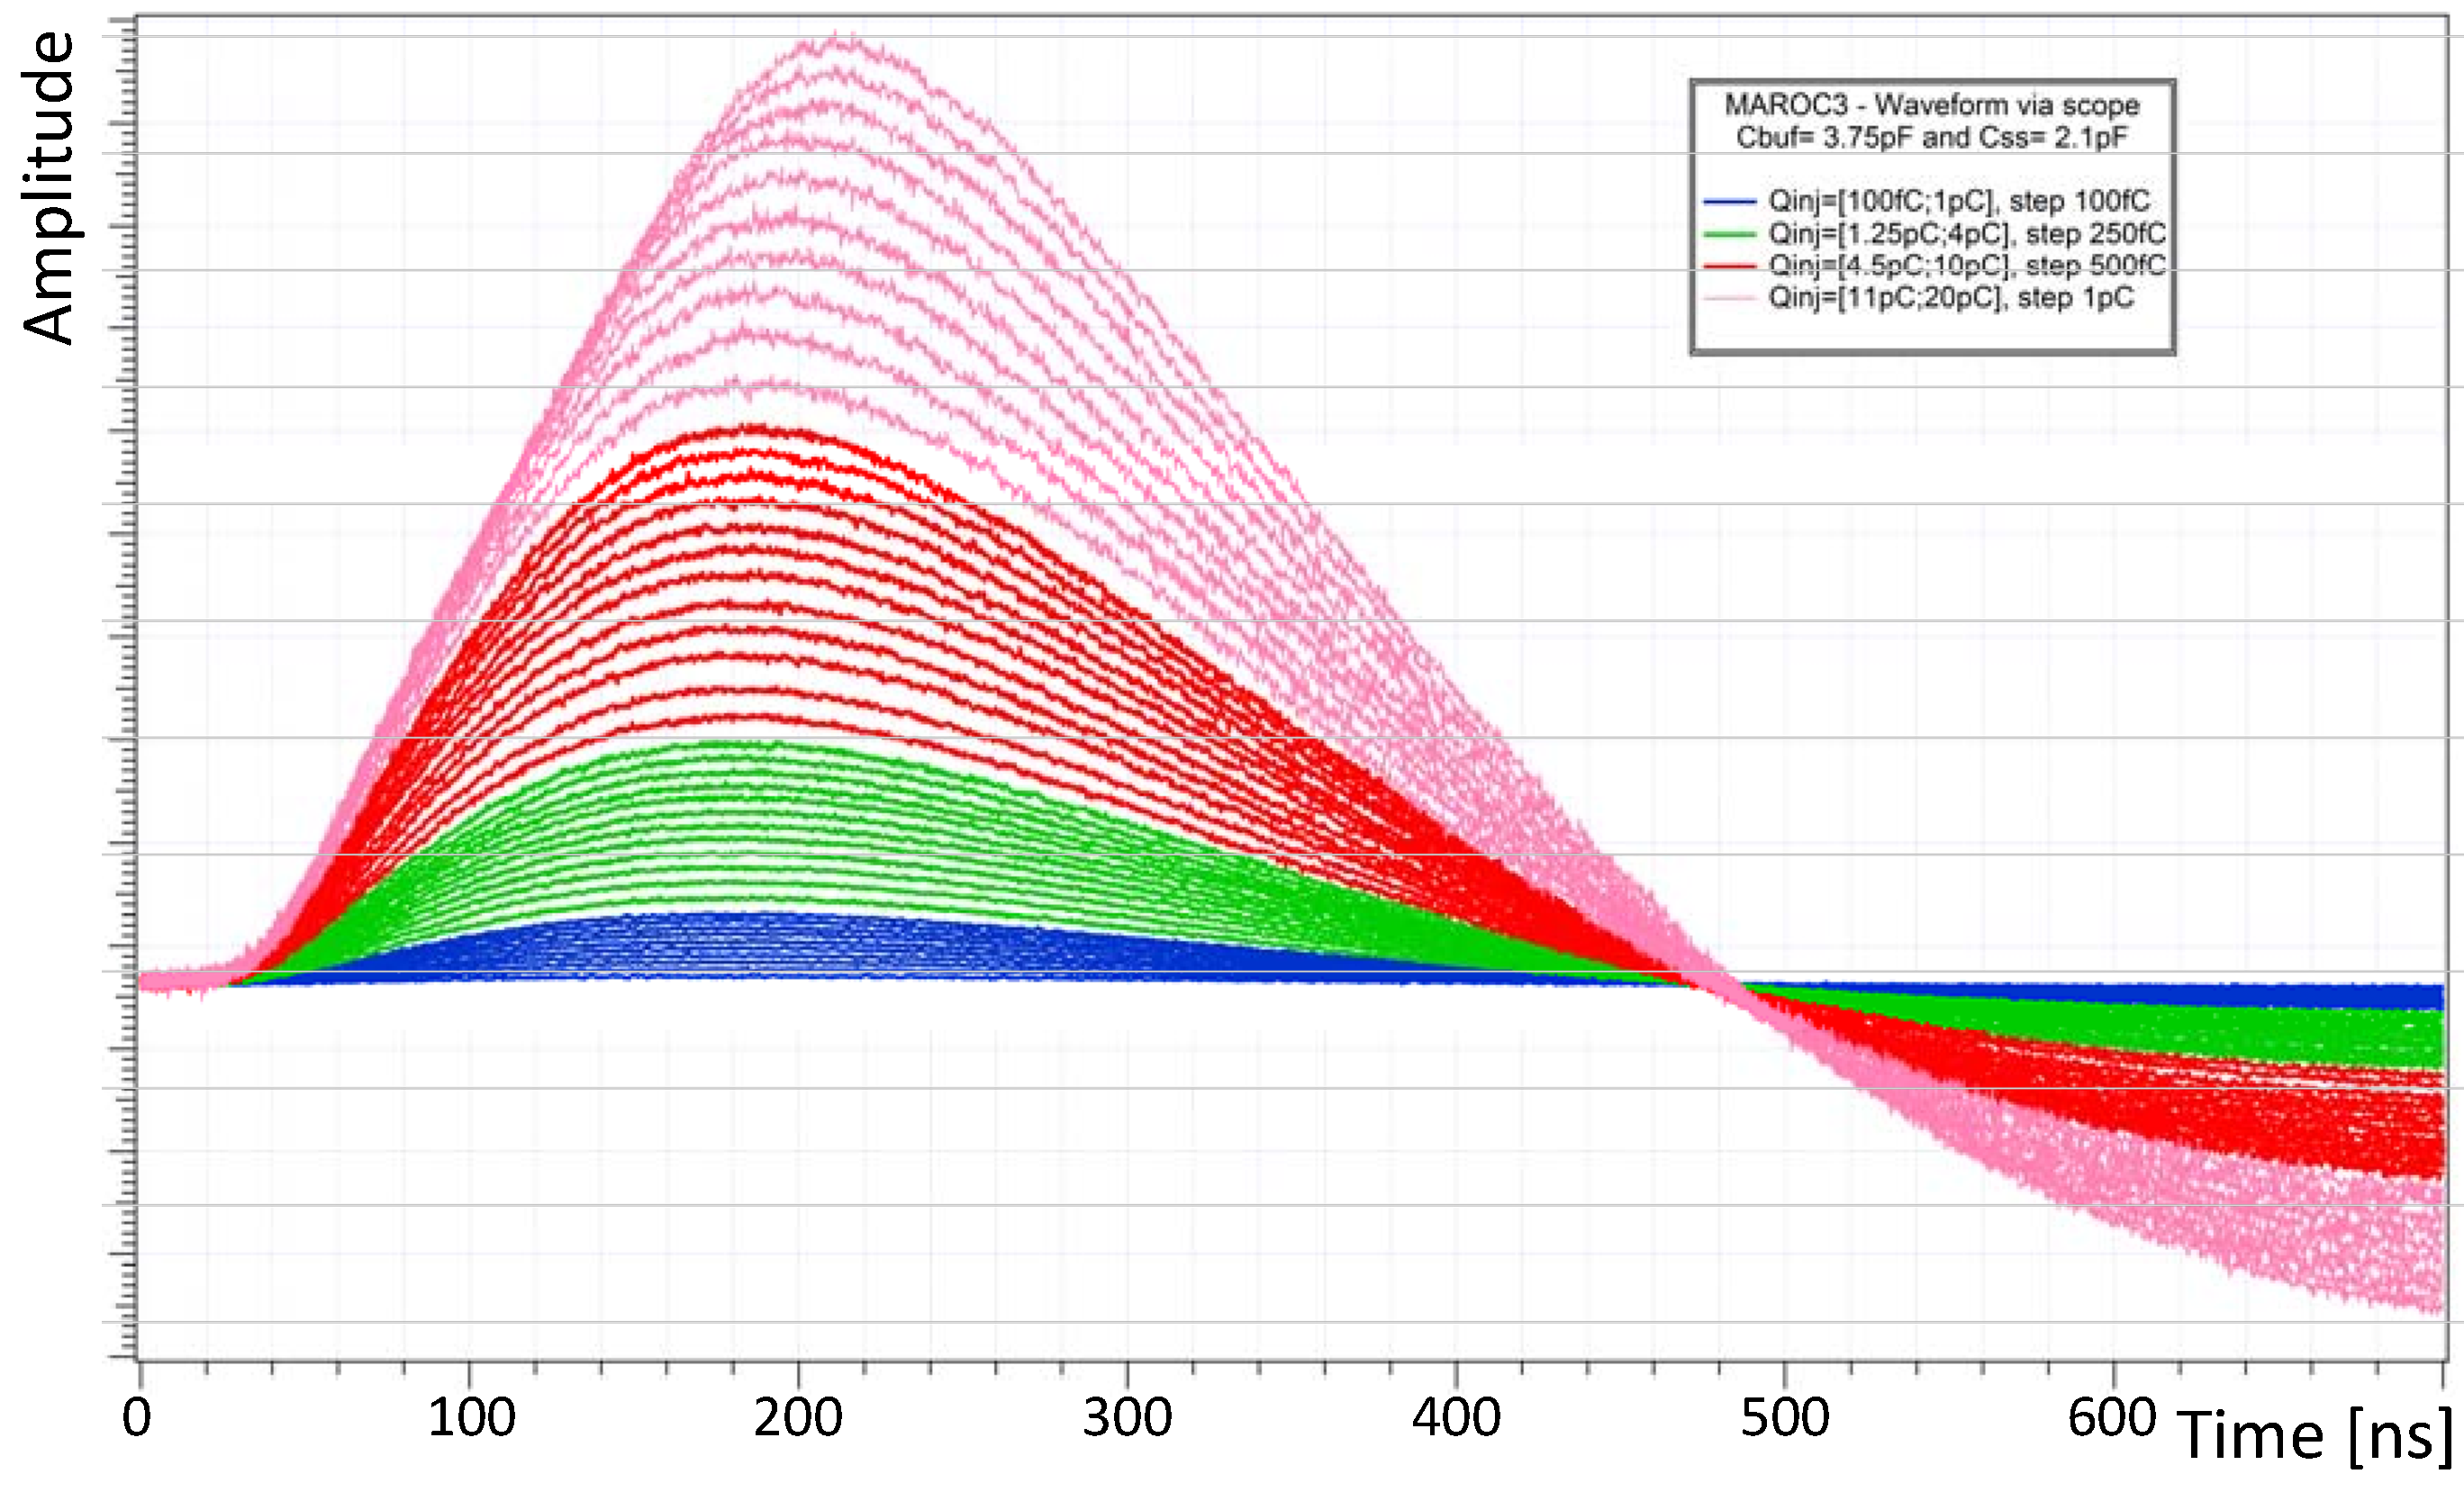
\includegraphics[width=\linewidth]{figures/SlowWaveForm_MAROC.pdf}
		\caption{Slow shaper waveform from MAROC datasheet for different charge injections}
		\label{fig:slowMAROC}
	\end{subfigure}
	\begin{subfigure}{0.49\linewidth}
		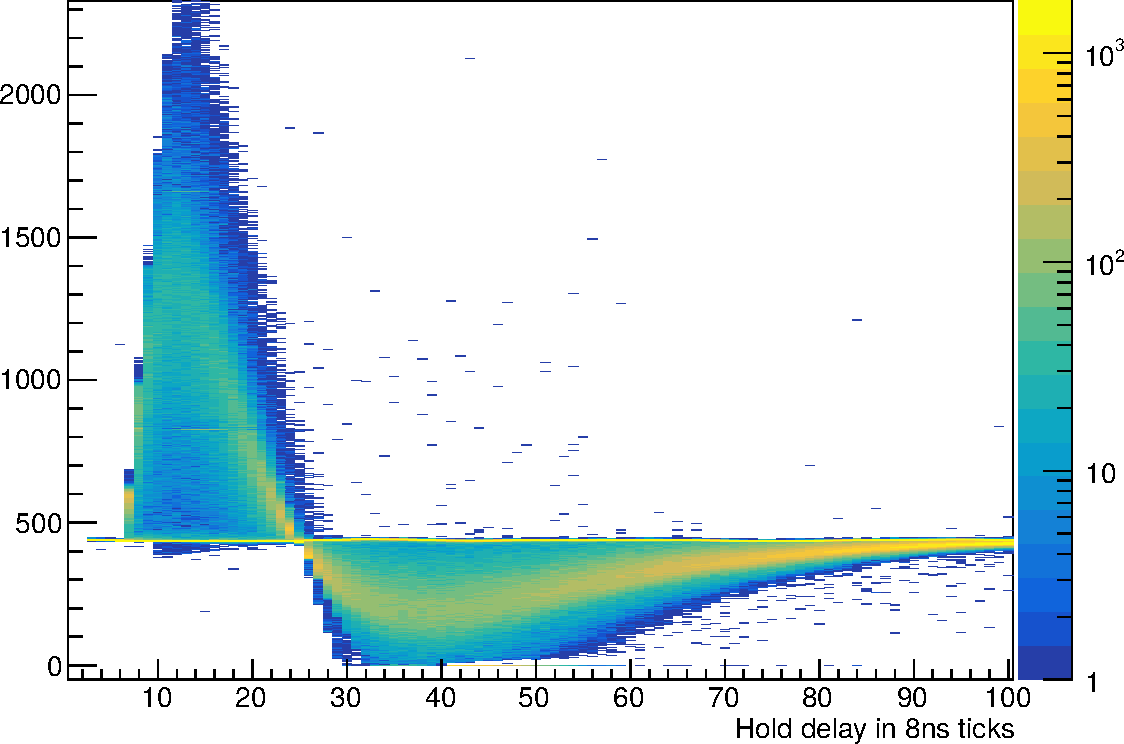
\includegraphics[width=\linewidth]{figures/SlowWaveForm_RICH.pdf}
		\caption{Slow shaper waveform from JLab data for MAPMT signal}
		\label{fig:slowJLab}
	\end{subfigure}
	\caption{Slow shaper response from MAROC}
	\label{fig:slowWaveform}
\end{figure}



\begin{figure}[hbt]
	\centering
	\begin{subfigure}{0.9\linewidth}
		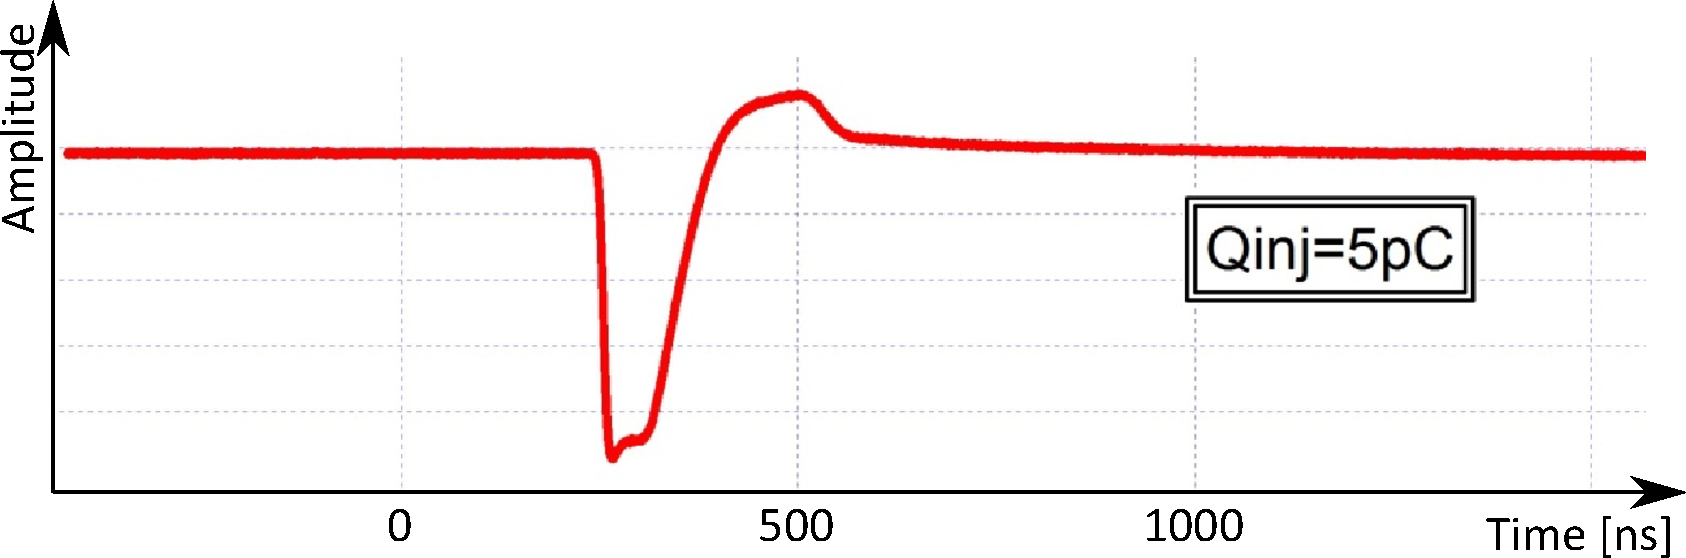
\includegraphics[width=\linewidth]{figures/FastShaper_MAROC.pdf}
		\caption{Fast shaper waveform from MAROC datasheet}
		\label{fig:fastMAROC}
	\end{subfigure}
	\begin{subfigure}{0.6\linewidth}
		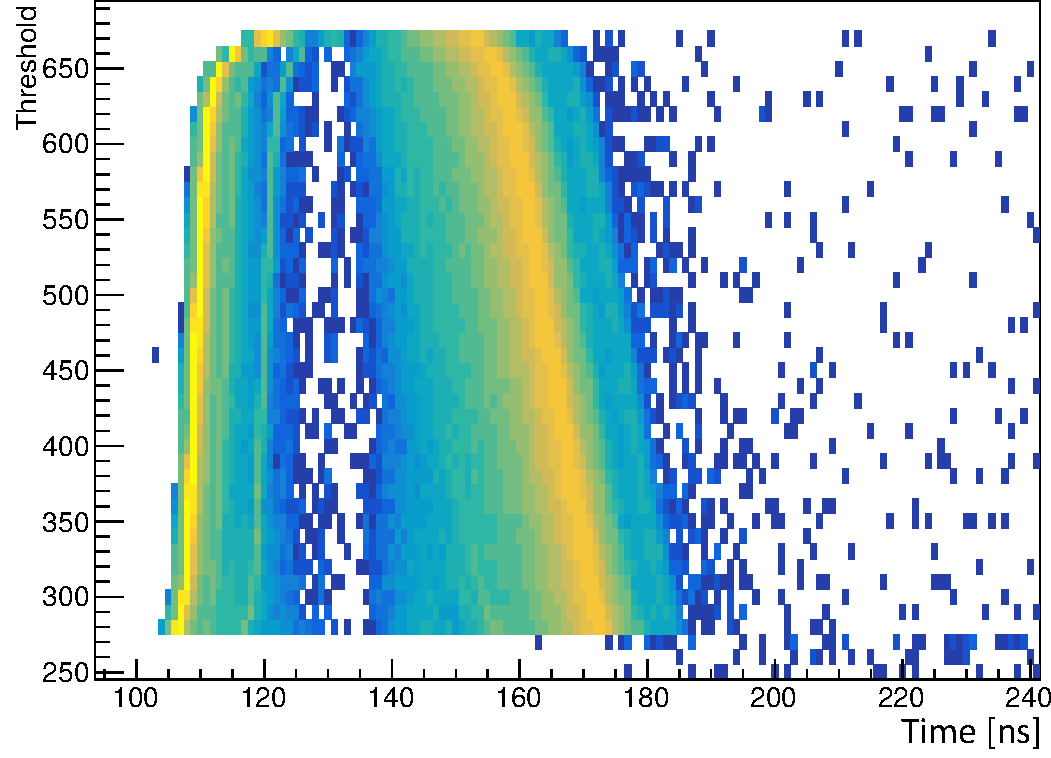
\includegraphics[width=\linewidth]{figures/FastWaveForm_RICH.pdf}
		\caption{Measured dependency of "time over threshold" vs threshold}
		\label{fig:fastJLab}
	\end{subfigure}
	\caption{Fast shaper response from MAROC}
	\label{fig:fastWaveform}
\end{figure}


The digital line can be sampled with a predefined clock on an adequate deep external digital pipeline with event information available promtly in parallel making it suitable for the RICH application.
The binary information comes from the discrimination of the fast shaper lines output.
On Fig.~\ref{fig:fastMAROC} the fast shaper waveform is shown for fixed injected charge from MAROC3 datasheet.
On the right fig.~\ref{fig:fastJLab} shows the the dependence of time over threshold versus threshold values.
The digital line reports the time when fast shaper waveform crosses the thhreshold value giving us the leading and trailing edges.
To reconstruct fast shaper waverform the measurements with different threshold values were collected and the time of leading and trailing edges were plotted.
As expected at higher thresholds the signal crosses the threhold later and has a shorter time over threshold.
Also the spread of SPE response from MAPMT gives us preliminary indication of signal's time walk which can be further corrected to improve time resolution.
The behaviour at high threshold might not represent the expected performance because the signal reaches saturation and loses its linearity.


Preliminary measurements of MAROC3 and MAPMTs demonstrate good time and charge resolution allowing to further improve our MAPMTs measurements and their understanding.
The final production of FE boards in nearly complete and we expect to start receiving FE tiles within the next month.
